
\section{RESULTS}

\subsection{Simulation variant 1 (selection method)}

Figure~\ref{selectionMethodBoxplot} presents a notched boxplot of the time to
convergence for the \textbf{selection with replacement} vs. \textbf{selection
without replacement} trials, with the \textsl{influence direction} variable
held constant at \textbf{neighbor influences node}. Clearly the \textbf{with
replacement} variant ($M$=1.2, $SD$=1.2) takes significantly longer to
converge than does \textbf{without replacement} ($M$=1.2, $SD$=1.2), as a
t-test for the difference of means confirms (t(15)=4.0, p=.001).

\begin{figure}[!tbp]
  \centering
  \subfloat[\textsl{Selection method} levels, with \textsl{influence
direction} set to \textbf{neighbor influences node}.]{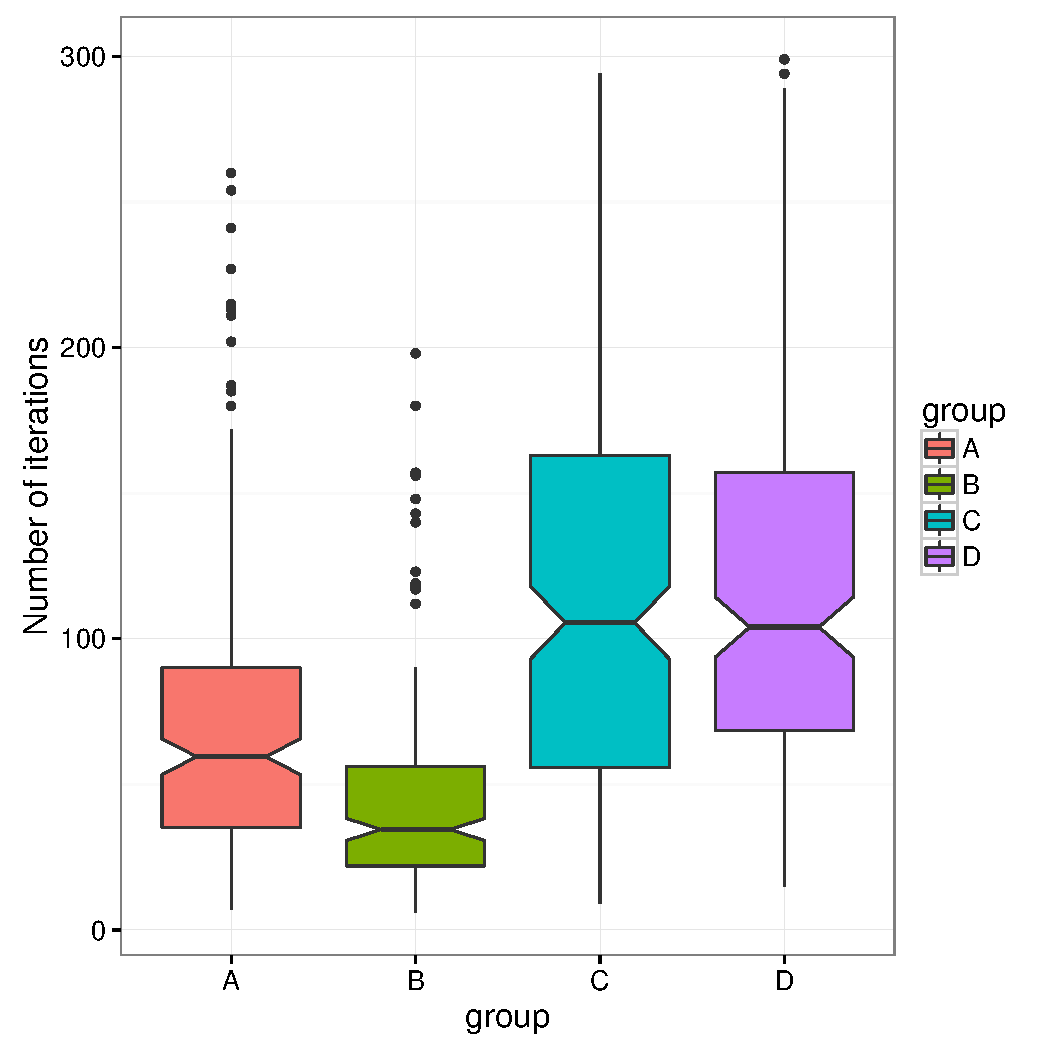
\includegraphics[width=0.4\textwidth]{selectionMethodBoxplot.pdf}\label{selectionMethodBoxplot}}
  \hfill
  \subfloat[\textsl{Influence direction} levels, with \textsl{selection
method} set to \textbf{without replacement}.]{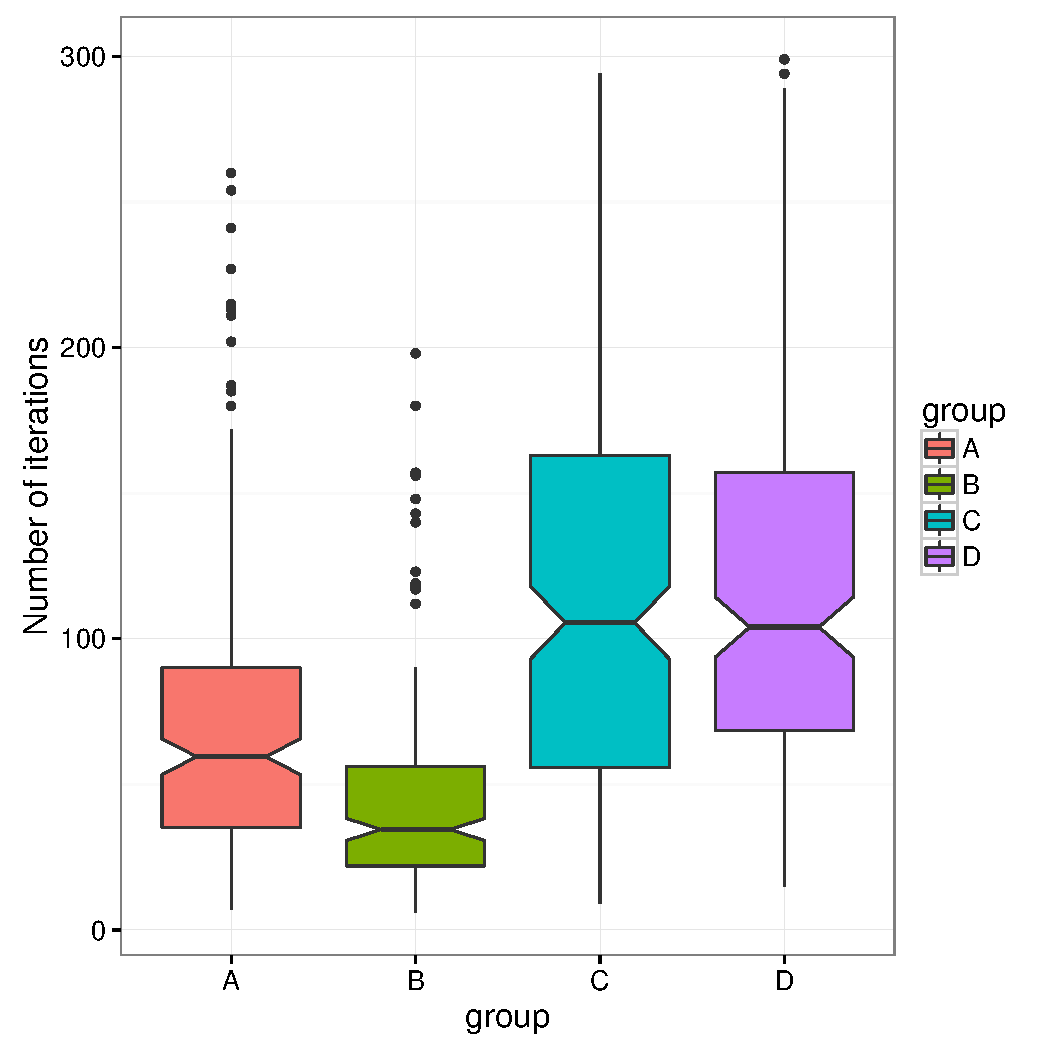
\includegraphics[width=0.4\textwidth]{influenceDirectionBoxplot.pdf}\label{influenceDirectionBoxplot}}
  \caption{Time to convergence of uniformity of opinion (N=400).}
\end{figure}


The explanation for this difference would appear to be the following. If the
nodes to be influenced are selected \textit{with} replacement, then inevitably
some nodes will have their opinions updated multiple times while others are
relatively inactive. Thus the permeation of the to-be-dominant opinion is
uneven: the contagion reaches and ``converts" some parts of the graph long
before the ``starved" nodes are influenced. Conversely, if chosen without
replacement, every node in the graph regularly has a chance to be influenced,
which means no hold outs can ``hide" in the graph.

% This is confirmed (?) by counting how many encounters actually result in
% conversions.




\subsection{Simulation variant 2 (influence direction)}

Similarly, a significant difference in convergence time exists between the
\textbf{neighbor influences node} ($M$=1.1, $SD$=1.1) and \textbf{node
influences neighbor} ($M$=1.1, $SD$=1.1) variants, this time holding
\textsl{selection method} constant at \textbf{selection without replacement}
(see Figure~\ref{influenceDirectionBoxplot}.) A t-test for the difference
between these means yields t(15)=4.0, p=.001.

Such a trivial implementation choice about the direction of information flow 
in a pairwise interaction yields unexpected results. On average, when the 
agents are victims, complete consensus is reached faster then when the agents
are influencers. Our iterpretation of this phenomenon pertains to the degree
of neighbors an agent has. When each agent is always doing the influencing, 
he will only have impact over agents' opinions with whom he is connected. 
Therefore, agents with a higher degree of edges are influenced the most
often. An agent is restricted to only influence a subset of the nodes
(i.e. his neighbors) in the graph on each cycle. This minor implementation
choice is effectively biased toward choosing higher-degree nodes. As a result,
nodes with lower-degrees have significantly less probability of changing. 
Acting in a similar fashion as stubborn nodes (Yildiz), we observed a slower, 
if at all, rate of convergence time.

Perhaps a resolution could be found in random sampling whether the agent is chosen 
to be the victim or influencer for every iteration?


\subsection{Variable interactions}

Finally, we point out a non-trivial interaction between the two factors. As
illustrated in Figure~\ref{interactionBoxplot}, the difference in convergence
times between the two \textsl{selection method}s is only significant when
\textbf{neighbor influences node}.

\begin{figure}[ht]
\centering
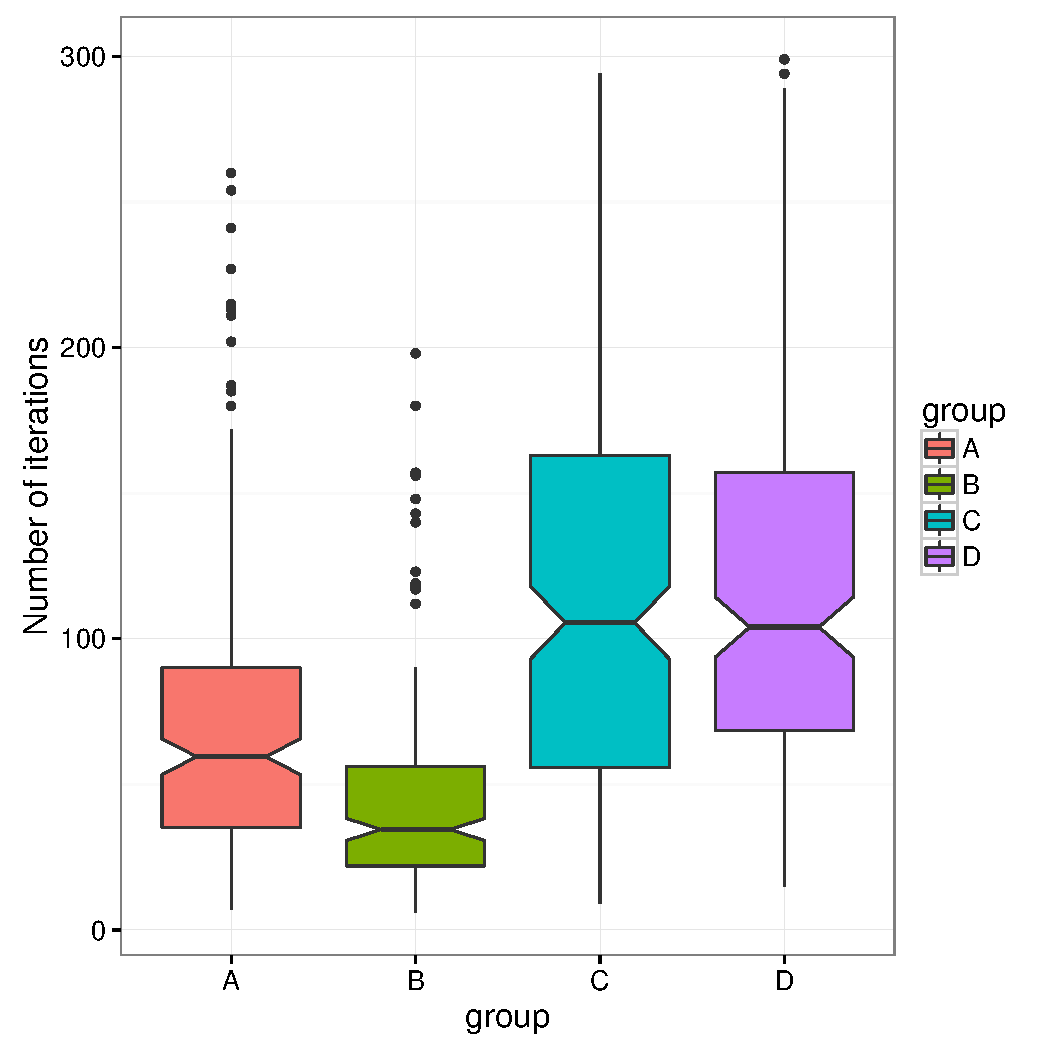
\includegraphics[width=0.45\textwidth]{interactionBoxplot.pdf} 
\caption{Full factorial design results for all four groups, illustrating
interaction between effects (N=800).}
\label{interactionBoxplot}
\end{figure}


